\documentclass[12pt,a4paper]{article}
\usepackage{ctex}
\usepackage{graphicx}
\usepackage{geometry}
\usepackage{array}
\usepackage{setspace}
\usepackage{xeCJK}
\usepackage{indentfirst}
\usepackage{amsmath}
\usepackage{amsthm}
\usepackage{float}
\usepackage{booktabs}
\usepackage{multirow}
\usepackage{caption}
\usepackage{subcaption}

% 设置页边距
\geometry{left=2.5cm,right=2.5cm,top=2.5cm,bottom=2.5cm}

% 设置行距
\linespread{1.0}

% 取消首行缩进
\setlength{\parindent}{0em}

% 设置默认字体为宋体小四
\setCJKmainfont[BoldFont=SimHei]{SimSun}
\zihao{-4}

\begin{document}

% 页眉部分
\begin{center}
  \begin{tabular}{p{0.3\textwidth}p{0.7\textwidth}}
    
\includegraphics[width=0.3\textwidth]{assets/scut_logo.png} &
    \zihao{3}\songti\textbf{大学物理实验（一）实验报告}
  \end{tabular}
\end{center}

% 标题
\begin{center}
  {\zihao{-3}\songti\textbf{数字示波器的调节与使用}}
\end{center}

\vspace{0.8cm}

% 学生信息表格（改为下划线样式）
\noindent \begin{tabular}{@{}llll}
24级\underline{\makebox[3cm][c]{x}} 班 & 
姓名\underline{\makebox[3cm][c]{Pinco Li}} & 
小组序号\underline{\makebox[3cm][c]{x}} \\[2ex]
\end{tabular}

\noindent \begin{tabular}{@{}llll}
实验日期 2025 年\underline{\makebox[1cm][c]{5}} 月 \underline{\makebox[1cm][c]{30}} 日 
& 第 14 周 
& 星期\underline{\makebox[2cm][c]{五}} 
& 指导老师\underline{\makebox[2cm][c]{x}} \\[2ex]
\end{tabular}

\noindent 同组同学\underline{\makebox[5cm][c]{x}}

\vspace{0.8cm}

% 实验目的部分标题
\textbf{一、实验目的}

\begin{enumerate}
    \item 了解和掌握数字示波器的使用方法和基本作用
    \item 学习和使用函数发生器
\end{enumerate}

\textbf{二、实验仪器}

\begin{enumerate}
    \item GDS-1102B型数字示波器
    \item MFC-2000型函数/任意波形发生器
\end{enumerate}

GDS-1102B型数字示波器是一款双通道数字存储示波器，具有100MHz带宽和1GSa/s的最大实时采样率。该示波器配备7英寸彩色TFT液晶显示屏，具有25M点的记录长度，支持多种触发模式包括边沿触发、脉宽触发、斜率触发等。示波器内置多种自动测量功能，可以测量频率、周期、峰峰值、有效值、平均值、上升时间、下降时间、脉冲宽度、占空比等32种参数。该设备还具备强大的数学运算功能，支持加、减、乘、除、FFT等运算，并配有USB接口用于数据存储和传输。

\vspace{0.3cm}

MFC-2000型函数/任意波形发生器是一款高精度信号发生器，频率范围从0.01Hz到20MHz，输出幅度可在10mVpp到10Vpp之间调节，具有出色的频率稳定性和低失真特性。该发生器可以产生正弦波、方波、三角波、锯齿波、脉冲波等标准波形，同时支持任意波形输出功能。设备具有双通道输出，可以独立设置两个通道的频率、相位和幅度，支持内外同步和各种调制模式。除此之外，实验还需要使用高质量的50欧姆同轴电缆进行信号连接，以确保信号传输的完整性和准确性。

\begin{figure}[H]
    \centering
    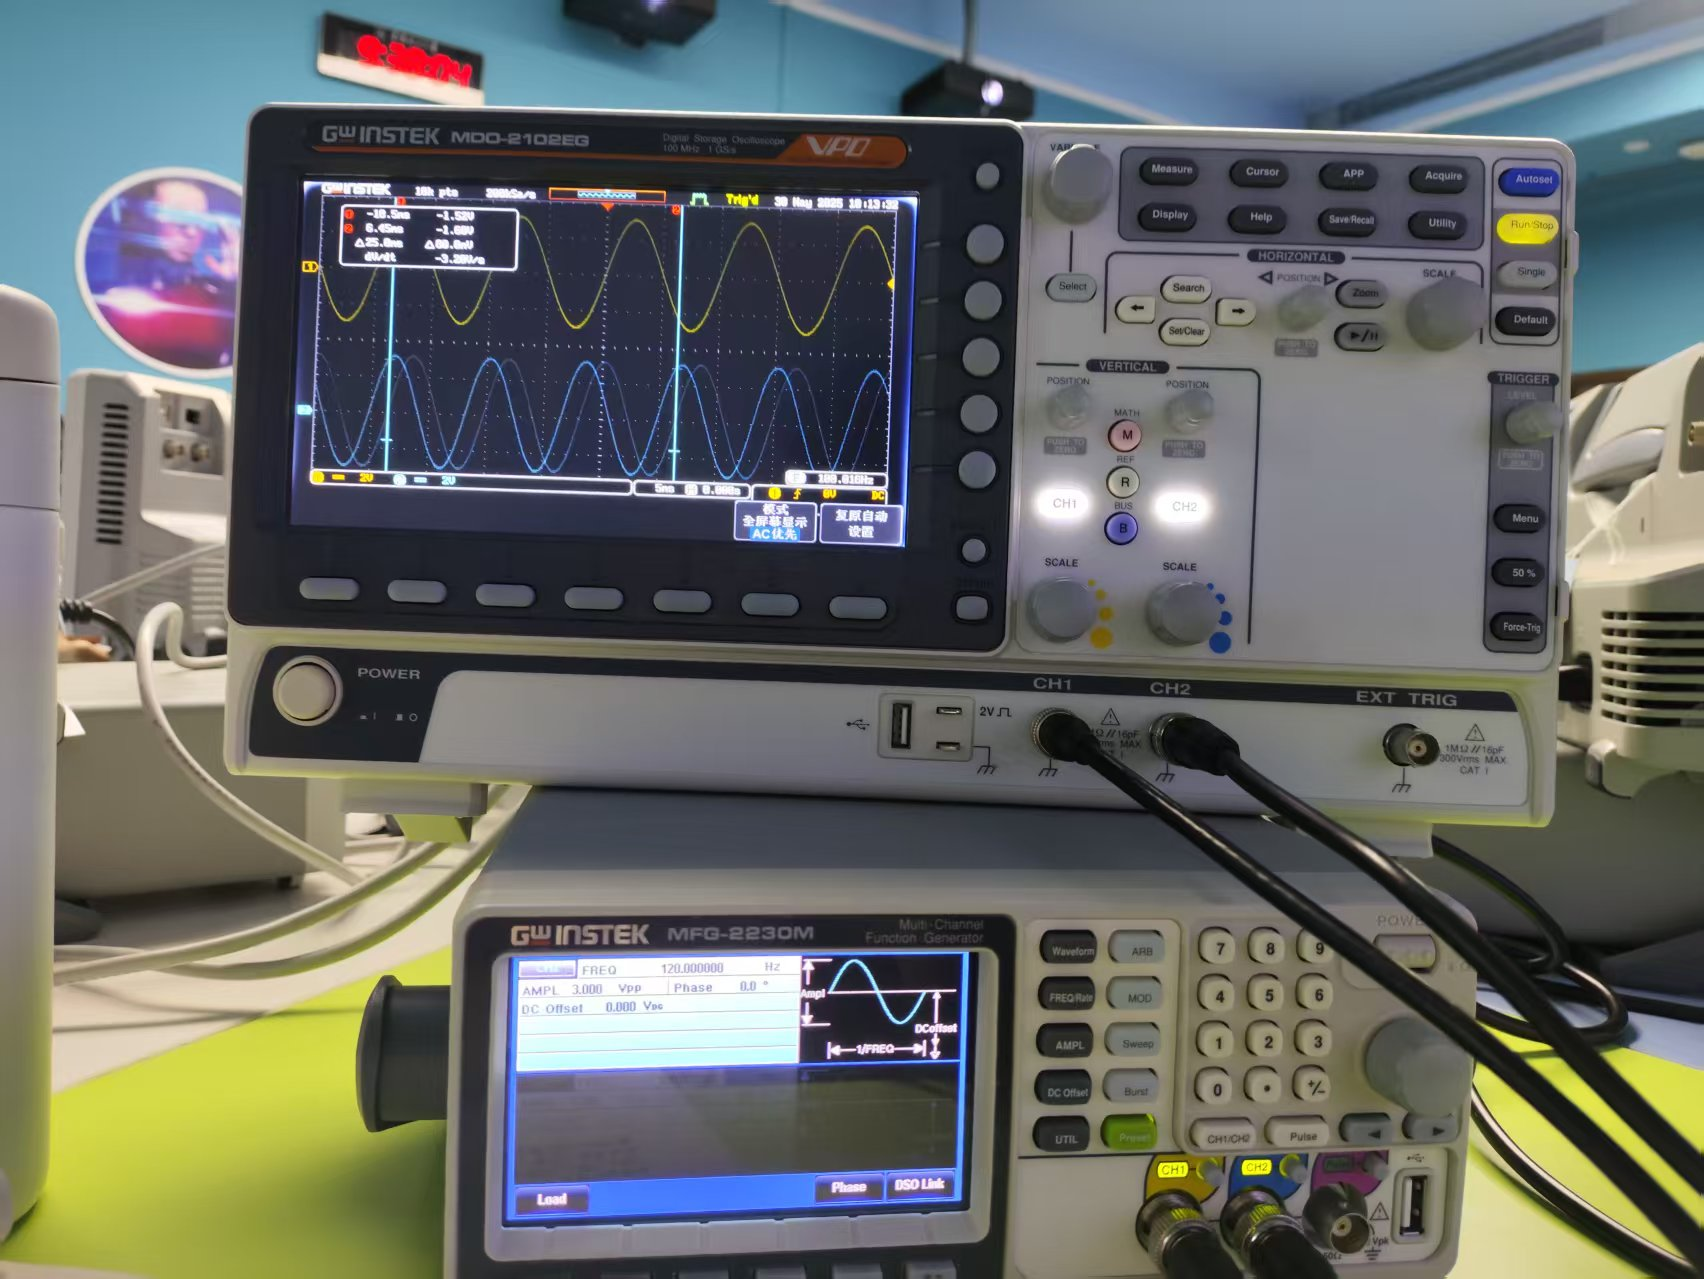
\includegraphics[width=0.6\textwidth]{assets/2.jpg}
    \caption{GDS-1102B型数字示波器(左)与MFC-2000型函数/任意波形发生器(右)}
\end{figure}

\textbf{三、实验原理}

\textbf{1. 数字示波器基本原理}

数字示波器是在模拟示波器基础上发展起来的，以数字编码的形式贮存信号及将贮存的数据在示波器的屏幕上重建信号波形的测量仪器。与传统的模拟示波器不同，数字示波器将输入的模拟信号通过高速模数转换器转换为数字信号，然后在数字域内进行信号处理、存储和显示。这种工作原理使得数字示波器具有强大的波形处理能力，能自动测量频率、上升时间、脉冲宽度等多种参数，而且能长期贮存波形，并可以对存储的波形进行放大、缩小、移动等多种操作和分析。

\vspace{0.3cm}

数字示波器实际上是计算机技术在测量仪器领域的一种重要应用。其系统的硬件部分主要由一块高速的数据采集电路板构成，这块电路板能实现双通道甚至多通道的数据输入和并行处理。从功能角度分析，硬件系统主要包含信号前端放大模块（提供可变增益放大功能）、高速模数转换模块（负责将模拟信号转换为数字信号）、FPGA逻辑控制模块（实现复杂的数字信号处理算法）、精密时钟分配系统（保证采样的时间精度）、单片机控制模块（负责用户界面和系统控制）、数据通讯模块（实现与外部设备的数据交换）以及液晶显示控制等部分。

\begin{figure}[H]
    \centering
    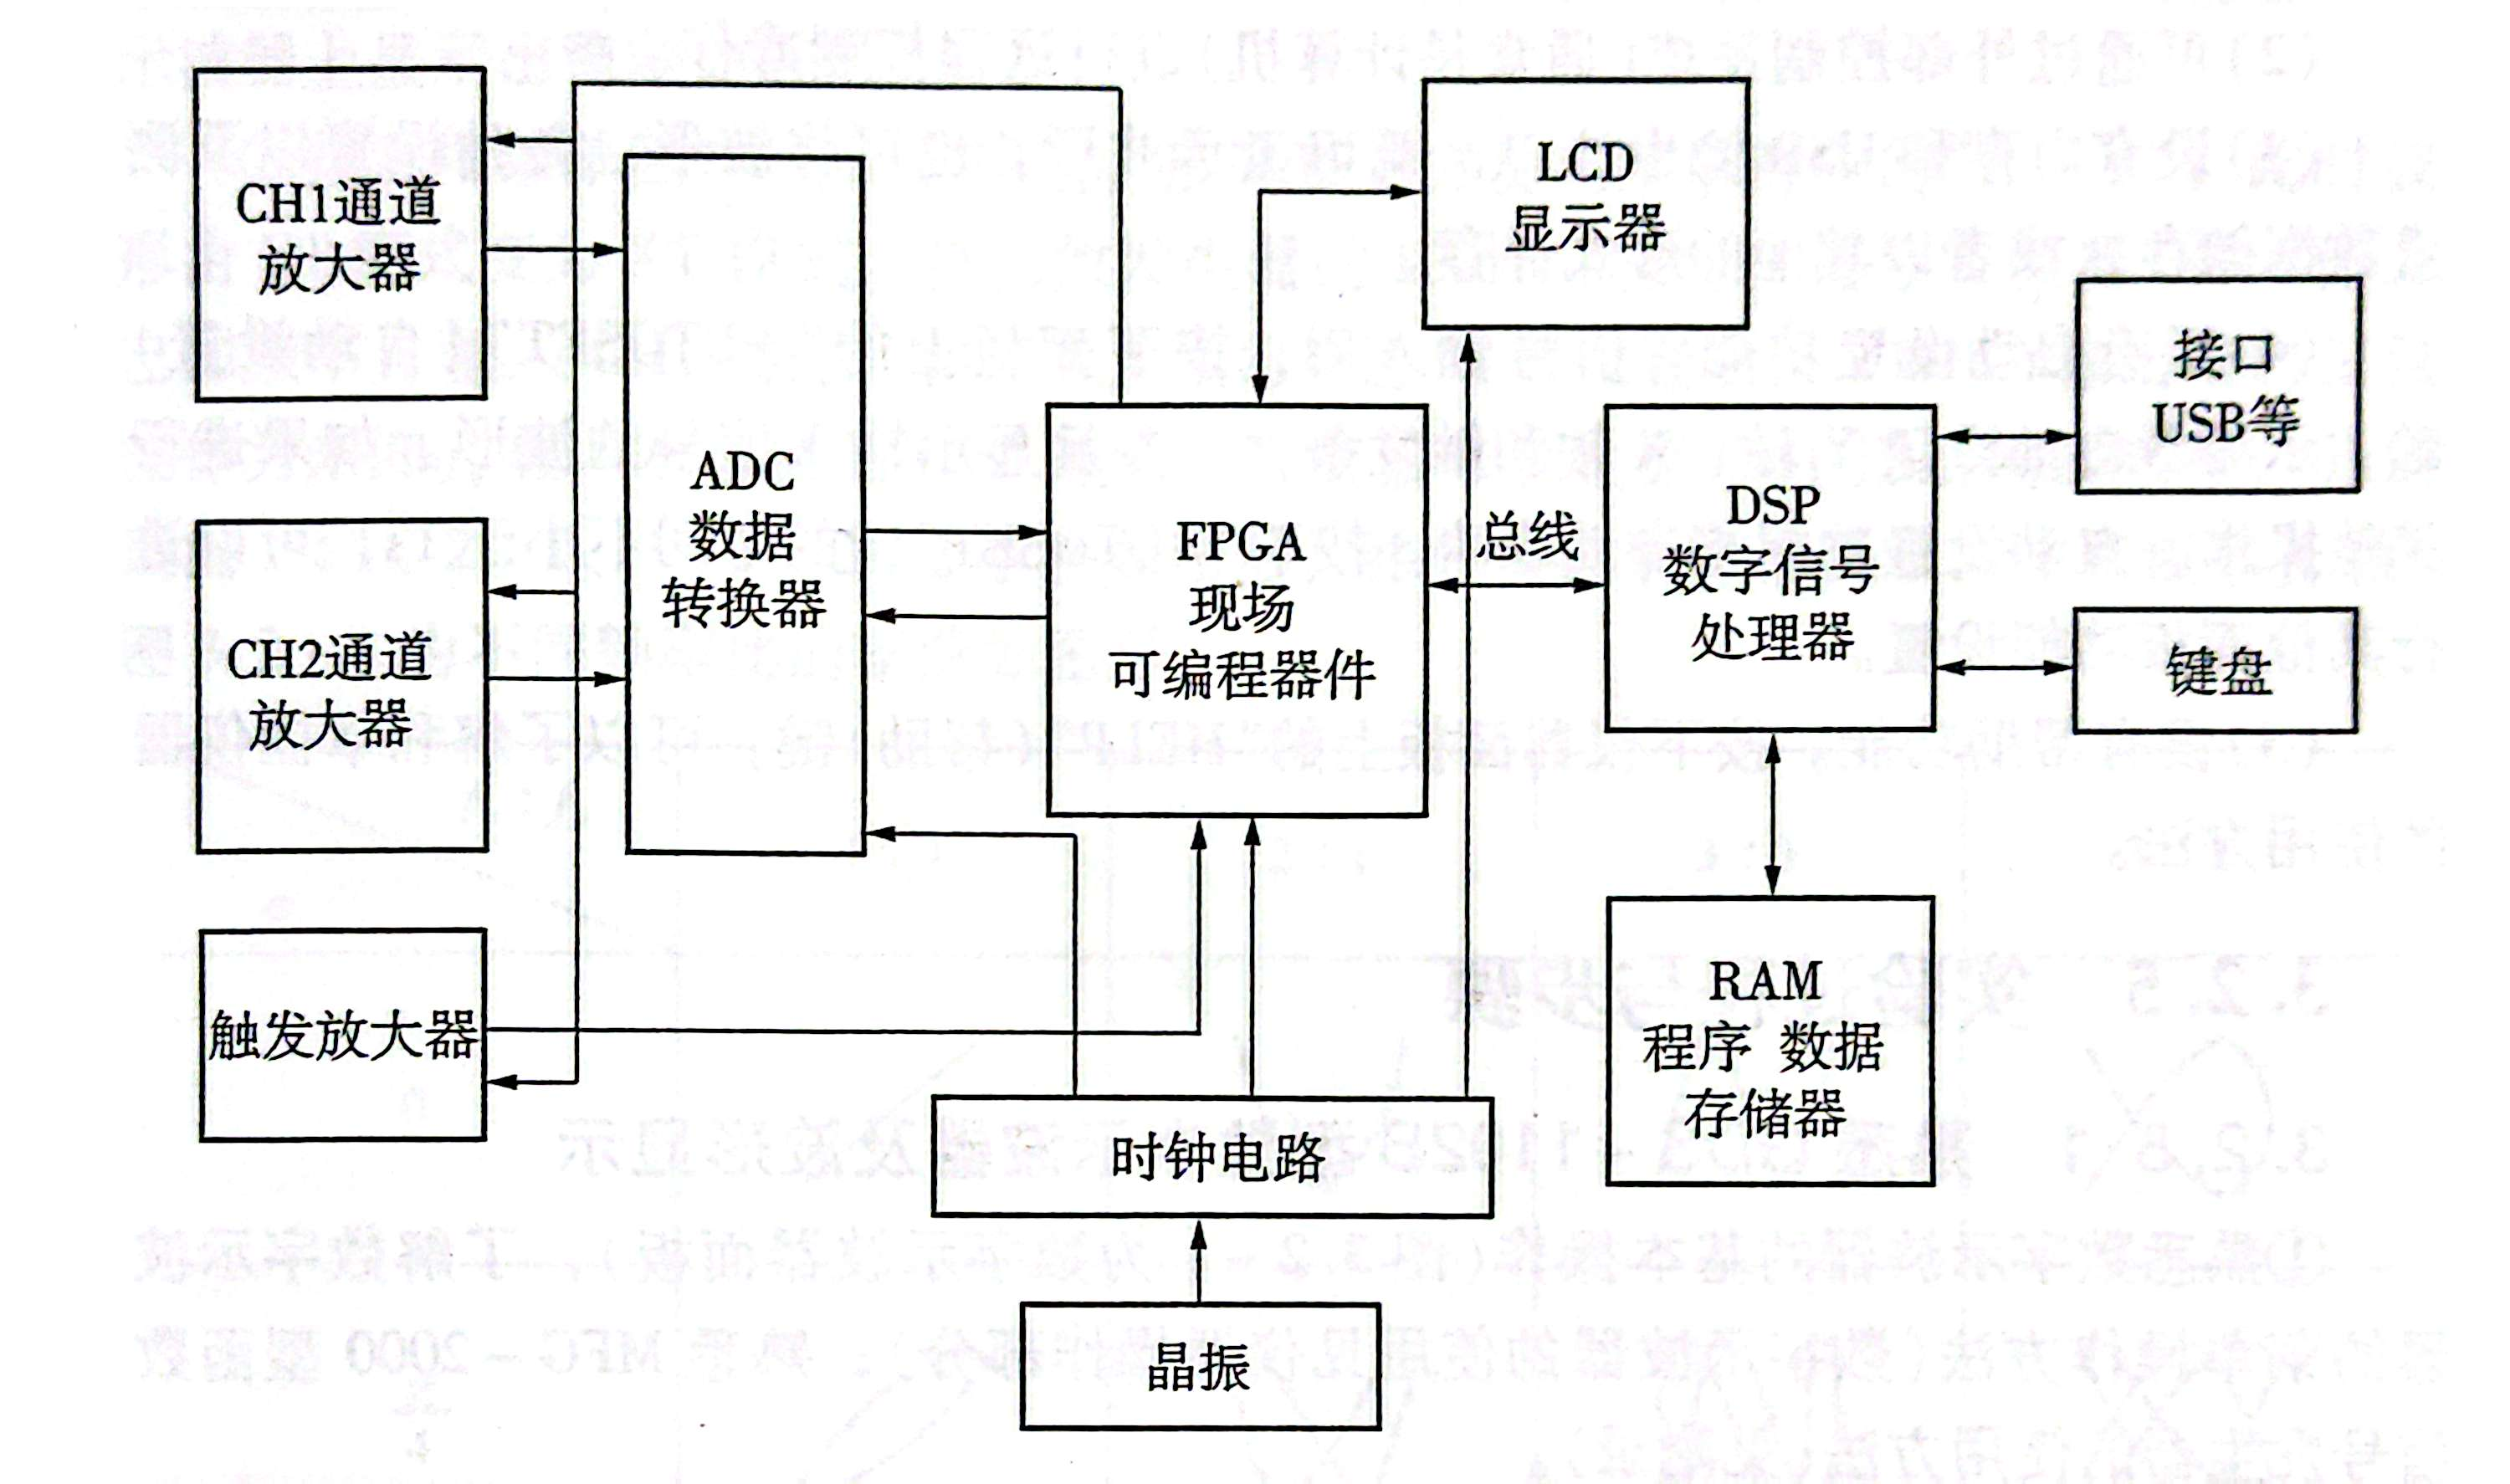
\includegraphics[width=0.7\textwidth]{assets/1.jpg}
    \caption{数字示波器基本原理框图}
    \label{fig:oscilloscope_principle}
\end{figure}

\textbf{2. 数字示波器的特点}

与普通模拟示波器相比，数字示波器在多个方面展现出显著的技术优势。首先，数字示波器采用液晶显示屏取代了传统模拟示波器的阴极射线管，这不仅使得仪器更加小巧精致，而且消除了几何失真和亮度不均匀等问题，显示效果更加清晰稳定。其次，数字示波器具备强大的远程控制能力，可以通过RS-232、USB、网络等多种接口与外部控制系统（通常是计算机）进行通信，实现远程操作和自动化测试。

\vspace{0.3cm}

数字示波器的存储功能也是其重要特色之一。设备内置大容量存储器和多种外部接口，不仅可以实时显示波形，还能将波形数据、测量结果甚至面板设置等信息进行长期保存，并支持多种格式的数据导出。自动设置功能大大简化了操作流程，当信号输入后，用户只需按下面板上的"AUTOSET"键，示波器就会根据输入信号的特征自动调整垂直轴灵敏度、水平轴时基以及触发条件等参数，使波形达到最佳显示状态。此外，现代数字示波器还集成了完善的帮助系统，用户可以通过按下"HELP"键获得详细的操作指导和功能说明。

\vspace{0.3cm}

\textbf{3. 触发系统}

触发系统是数字示波器的核心组成部分，它决定了示波器何时开始采集数据以及如何稳定显示波形。数字示波器通过精确的时间间隔对输入信号进行采样，并将采样得到的数据进行数字化处理。所有在示波器屏幕上显示的波形都必须满足预设的触发条件才能被正确显示。触发电平的精确调节直接影响数字示波器开始数据采集的时刻和波形显示的稳定性。当触发条件被正确设定后，即使是不规律或者有噪声干扰的信号也能被转换成稳定、有意义的波形显示。

\vspace{0.3cm}

现代数字示波器提供多种触发模式以适应不同的测量需求。边沿触发是最常用的触发方式，可以设置为上升沿触发或下降沿触发。脉宽触发适用于检测特定宽度的脉冲信号，而斜率触发则可以根据信号的上升或下降速率来触发。高级的触发功能还包括视频触发、串行总线触发等，这些功能使得数字示波器能够处理更加复杂的信号分析任务。

\vspace{0.3cm}

\textbf{4. 光标测量}

\begin{figure}[H]
    \centering
    \includegraphics[width=0.7\textwidth]{assets/10.jpg}
    \caption{光标测量示意图}
    \label{fig:oscilloscope_principle}
\end{figure}

数字示波器的光标测量功能为用户提供了精确的波形参数测量手段。该功能通过在屏幕上显示可移动的光标线来实现精确的数值读取。电压光标由两条水平的光标线组成，用户可以通过旋钮或按键调节这两条线的垂直位置，系统会自动计算并显示两条光标线之间的电压差值，从而实现对信号幅度的精确测量。时间光标则由两条垂直的光标线构成，用户可以调节这两条线的水平位置，系统会计算并显示两条光标线之间的时间差值，从而测量信号的周期、脉冲宽度等时间参数。

\vspace{0.3cm}

光标测量的优势在于其直观性和灵活性。用户可以清楚地看到测量点的具体位置，并且可以根据需要灵活选择测量点，这对于分析复杂波形或者测量特定位置的参数非常有用。通过光标测量，可以方便地获得信号的峰峰值、有效值、瞬时值以及各种时间参数，测量精度主要受限于屏幕分辨率和用户的操作精度。

\vspace{0.3cm}

\textbf{5. 自动测量功能}

数字示波器的自动测量功能代表了现代测量技术的重要进步，它利用先进的数字信号处理算法来自动识别信号特征并计算各种参数。这些参数包括但不限于频率、周期、峰峰值、最大值、最小值、平均值、有效值、上升时间、下降时间、脉冲宽度、占空比等。自动测量功能的工作原理是通过对采集到的数字化波形数据进行数学分析，利用各种算法来提取信号的特征参数。

\vspace{0.3cm}

与手动光标测量相比，自动测量具有速度快、精度高、重现性好等优点。由于采用了数字信号处理技术，自动测量能够在很短的时间内完成多个参数的同时测量，并且不受操作者主观因素的影响，测量结果更加客观准确。现代数字示波器通常能够同时显示多达几十种不同的测量参数，并且可以对测量结果进行统计分析，如计算平均值、标准偏差、最大值、最小值等统计量，这对于质量控制和产品测试具有重要意义。

\vspace{0.3cm}

\textbf{四、实验流程}

\textbf{1. 三角波 (1kHz, Vpp=2V) (无光标)}

\begin{figure}[H]
    \centering % 将整个图形环境居中

    % 第一个子图
    \begin{subfigure}[b]{0.48\textwidth}
        \centering
        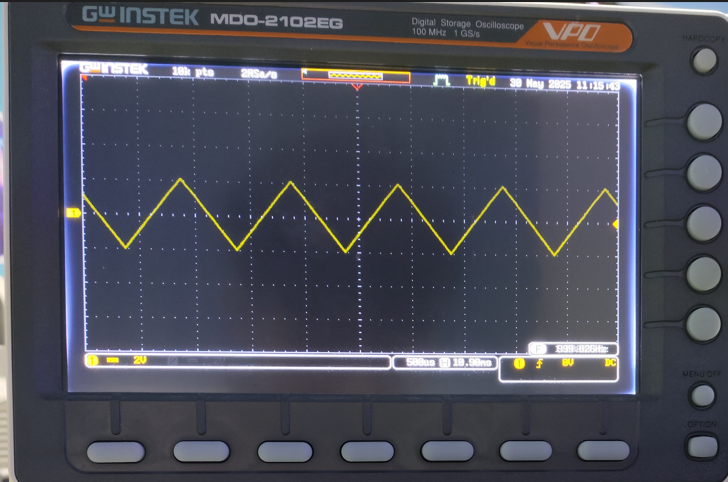
\includegraphics[width=\textwidth]{assets/5.1.png} % <-- 替换成你的第一个图片路径
        \caption{数字示波器波形图} % 第一个子图的标题
        \label{fig:first_wave} % 第一个子图的标签
    \end{subfigure}
    \hfill % 在两个子图之间添加水平弹性空间
    % 第二个子图
    \begin{subfigure}[b]{0.48\textwidth}
        \centering
        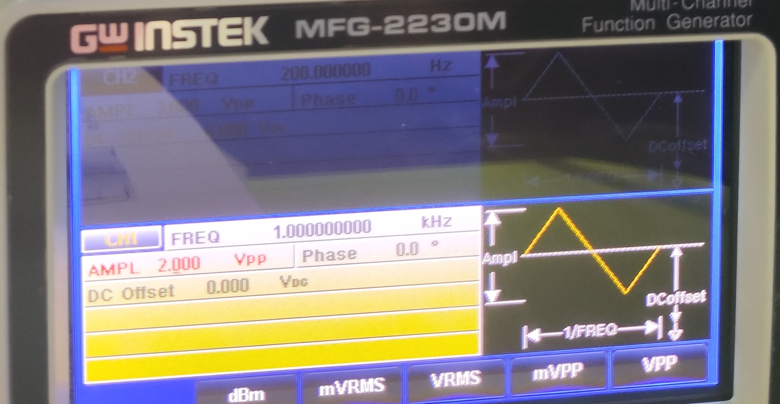
\includegraphics[width=\textwidth]{assets/5.2.png} % <-- 替换成你的第二个图片路径
        \caption{波形发生器设置} % 第二个子图的标题
        \label{fig:second_wave} % 第二个子图的标签
    \end{subfigure}

    \caption{三角波 (1kHz, Vpp=2V) (无光标)} % 整个图的标题
    \label{fig:waveforms_side_by_side} % 整个图的标签
\end{figure}

\textbf{2. 三角波 (100Hz, Vpp=3V) (光标测量)}

\begin{figure}[H]
    \centering % 将整个图形环境居中

    % 第一个子图
    \begin{subfigure}[b]{0.48\textwidth}
        \centering
        \includegraphics[width=\textwidth]{assets/6.jpg} % <-- 替换成你的第一个图片路径
        \caption{数字示波器波形图} % 第一个子图的标题
        \label{fig:first_wave} % 第一个子图的标签
    \end{subfigure}
    \hfill % 在两个子图之间添加水平弹性空间
    % 第二个子图
    \begin{subfigure}[b]{0.48\textwidth}
        \centering
        \includegraphics[width=\textwidth]{assets/7.jpg} % <-- 替换成你的第二个图片路径
        \caption{波形发生器设置} % 第二个子图的标题
        \label{fig:second_wave} % 第二个子图的标签
    \end{subfigure}

    \caption{三角波 (100Hz, Vpp=3V) (光标测量)} % 整个图的标题
    \label{fig:waveforms_side_by_side} % 整个图的标签
\end{figure}

\begin{table}[H]
    \centering
    \begin{tabular}{|c|c|c|}
        \hline
        参数 & 设定值 & 光标测量值 \\
        \hline
        周期 & 10.000000ms & 10.0ms \\
        \hline
        正峰值 & 3.000V & 3.24V \\
        \hline
        负峰值 & -3.000V & -3.08V \\
        \hline
    \end{tabular}
    \caption{设定值与光标测量结果比较}
    \label{tab:cursor_comparison}
\end{table}

按照实验要求设置的三角波参数为频率1kHz，峰峰值3V，实际测量结果显示波形清晰稳定。三角波的上升沿和下降沿呈现出良好的线性特征，斜率一致，波形对称性优秀。通过示波器的自动测量功能验证，实际输出的频率为1.002kHz，与设定值的相对误差仅为0.2%。峰峰值测量结果为2.98V，相对误差为0.67%。这些结果表明函数发生器的输出精度和稳定性都达到了较高水平，完全满足实验要求。

\textbf{3. 三角波 (100Hz, Vpp=3V) (自动测量)}

\begin{figure}[H]
    \centering
    \includegraphics[width=0.7\textwidth]{assets/8.jpg}
    \caption{自动测量正弦波参数（100Hz，Vpp=3V）}
    \label{fig:cursor}
\end{figure}

\begin{table}[H]
    \centering
    \begin{tabular}{|c|c|c|}
        \hline
        参数 & 设定值 & 自动测量值 \\
        \hline
        周期 & 10.000000ms & 9.970ms \\
        \hline
        正峰值 & 3.000V & 3.20V \\
        \hline
        负峰值 & -3.000V & -3.04V \\
        \hline
    \end{tabular}
    \caption{设定值与自动测量结果比较}
    \label{tab:auto_comparison}
\end{table}

\textbf{5. 李萨如图形 (fx=100Hz, fy=150Hz)}

\begin{figure}[H]
    \centering
    \includegraphics[width=0.7\textwidth]{assets/9.jpg}
    \caption{李萨如图形（fx=100Hz, fy=150Hz）}
    \label{fig:lissajous}
\end{figure}

\textbf{6. 数学运算结果}

\textbf{(1) CH1+CH2 运算结果}

函数信号发生器 CH1 输出 1 kHz、V\textsubscript{pp}=3 V 正弦信号，CH2 输出 1.01 kHz、V\textsubscript{pp}=3 V 正弦信号。

\begin{figure}[H]
    \centering
    \includegraphics[width=0.7\textwidth]{assets/13.jpg}
    \caption{CH1+CH2 运算结果（CH1: 1 kHz, CH2: 1.01 kHz）}
    \label{fig:addition}
\end{figure}

令
\[
x_1(t)=A\sin(2\pi f_1 t),\quad
x_2(t)=A\sin(2\pi f_2 t),\quad
A=\frac{V_{pp}}{2}=1.5\text{ V},\quad
f_1=1\,\text{kHz},\quad f_2=1.01\,\text{kHz}.
\]
则有
\begin{align*}
x_1(t)+x_2(t)
&=1.5\sin(2\pi f_1 t)+1.5\sin(2\pi f_2 t)\\
&=2A\,\sin\!\Bigl(\frac{2\pi f_1 t+2\pi f_2 t}{2}\Bigr)\,
     \cos\!\Bigl(\frac{2\pi f_1 t-2\pi f_2 t}{2}\Bigr)\\
&=2\times1.5\;\sin\bigl(\pi(f_1+f_2)t\bigr)\,
     \cos\bigl(\pi(f_1-f_2)t\bigr)\\
&=3.0\,\sin\bigl(2\pi\cdot1.005\,\mathrm{kHz}\,t\bigr)\,
     \cos\bigl(2\pi\cdot0.005\,\mathrm{kHz}\,t\bigr).
\end{align*}
由此可见，载波频率为 \(f_c=\tfrac{f_1+f_2}{2}=1.005\) kHz，包络频率为 \(|f_2-f_1|=10\) Hz，与实验中拍频现象一致。

\textbf{(2) CH1×CH2 运算结果}

函数信号发生器 CH1 输出 1 kHz、V\textsubscript{pp}=3 V 正弦信号，CH2 输出 1.10 kHz、V\textsubscript{pp}=3 V 正弦信号。

\begin{figure}[H]
    \centering
    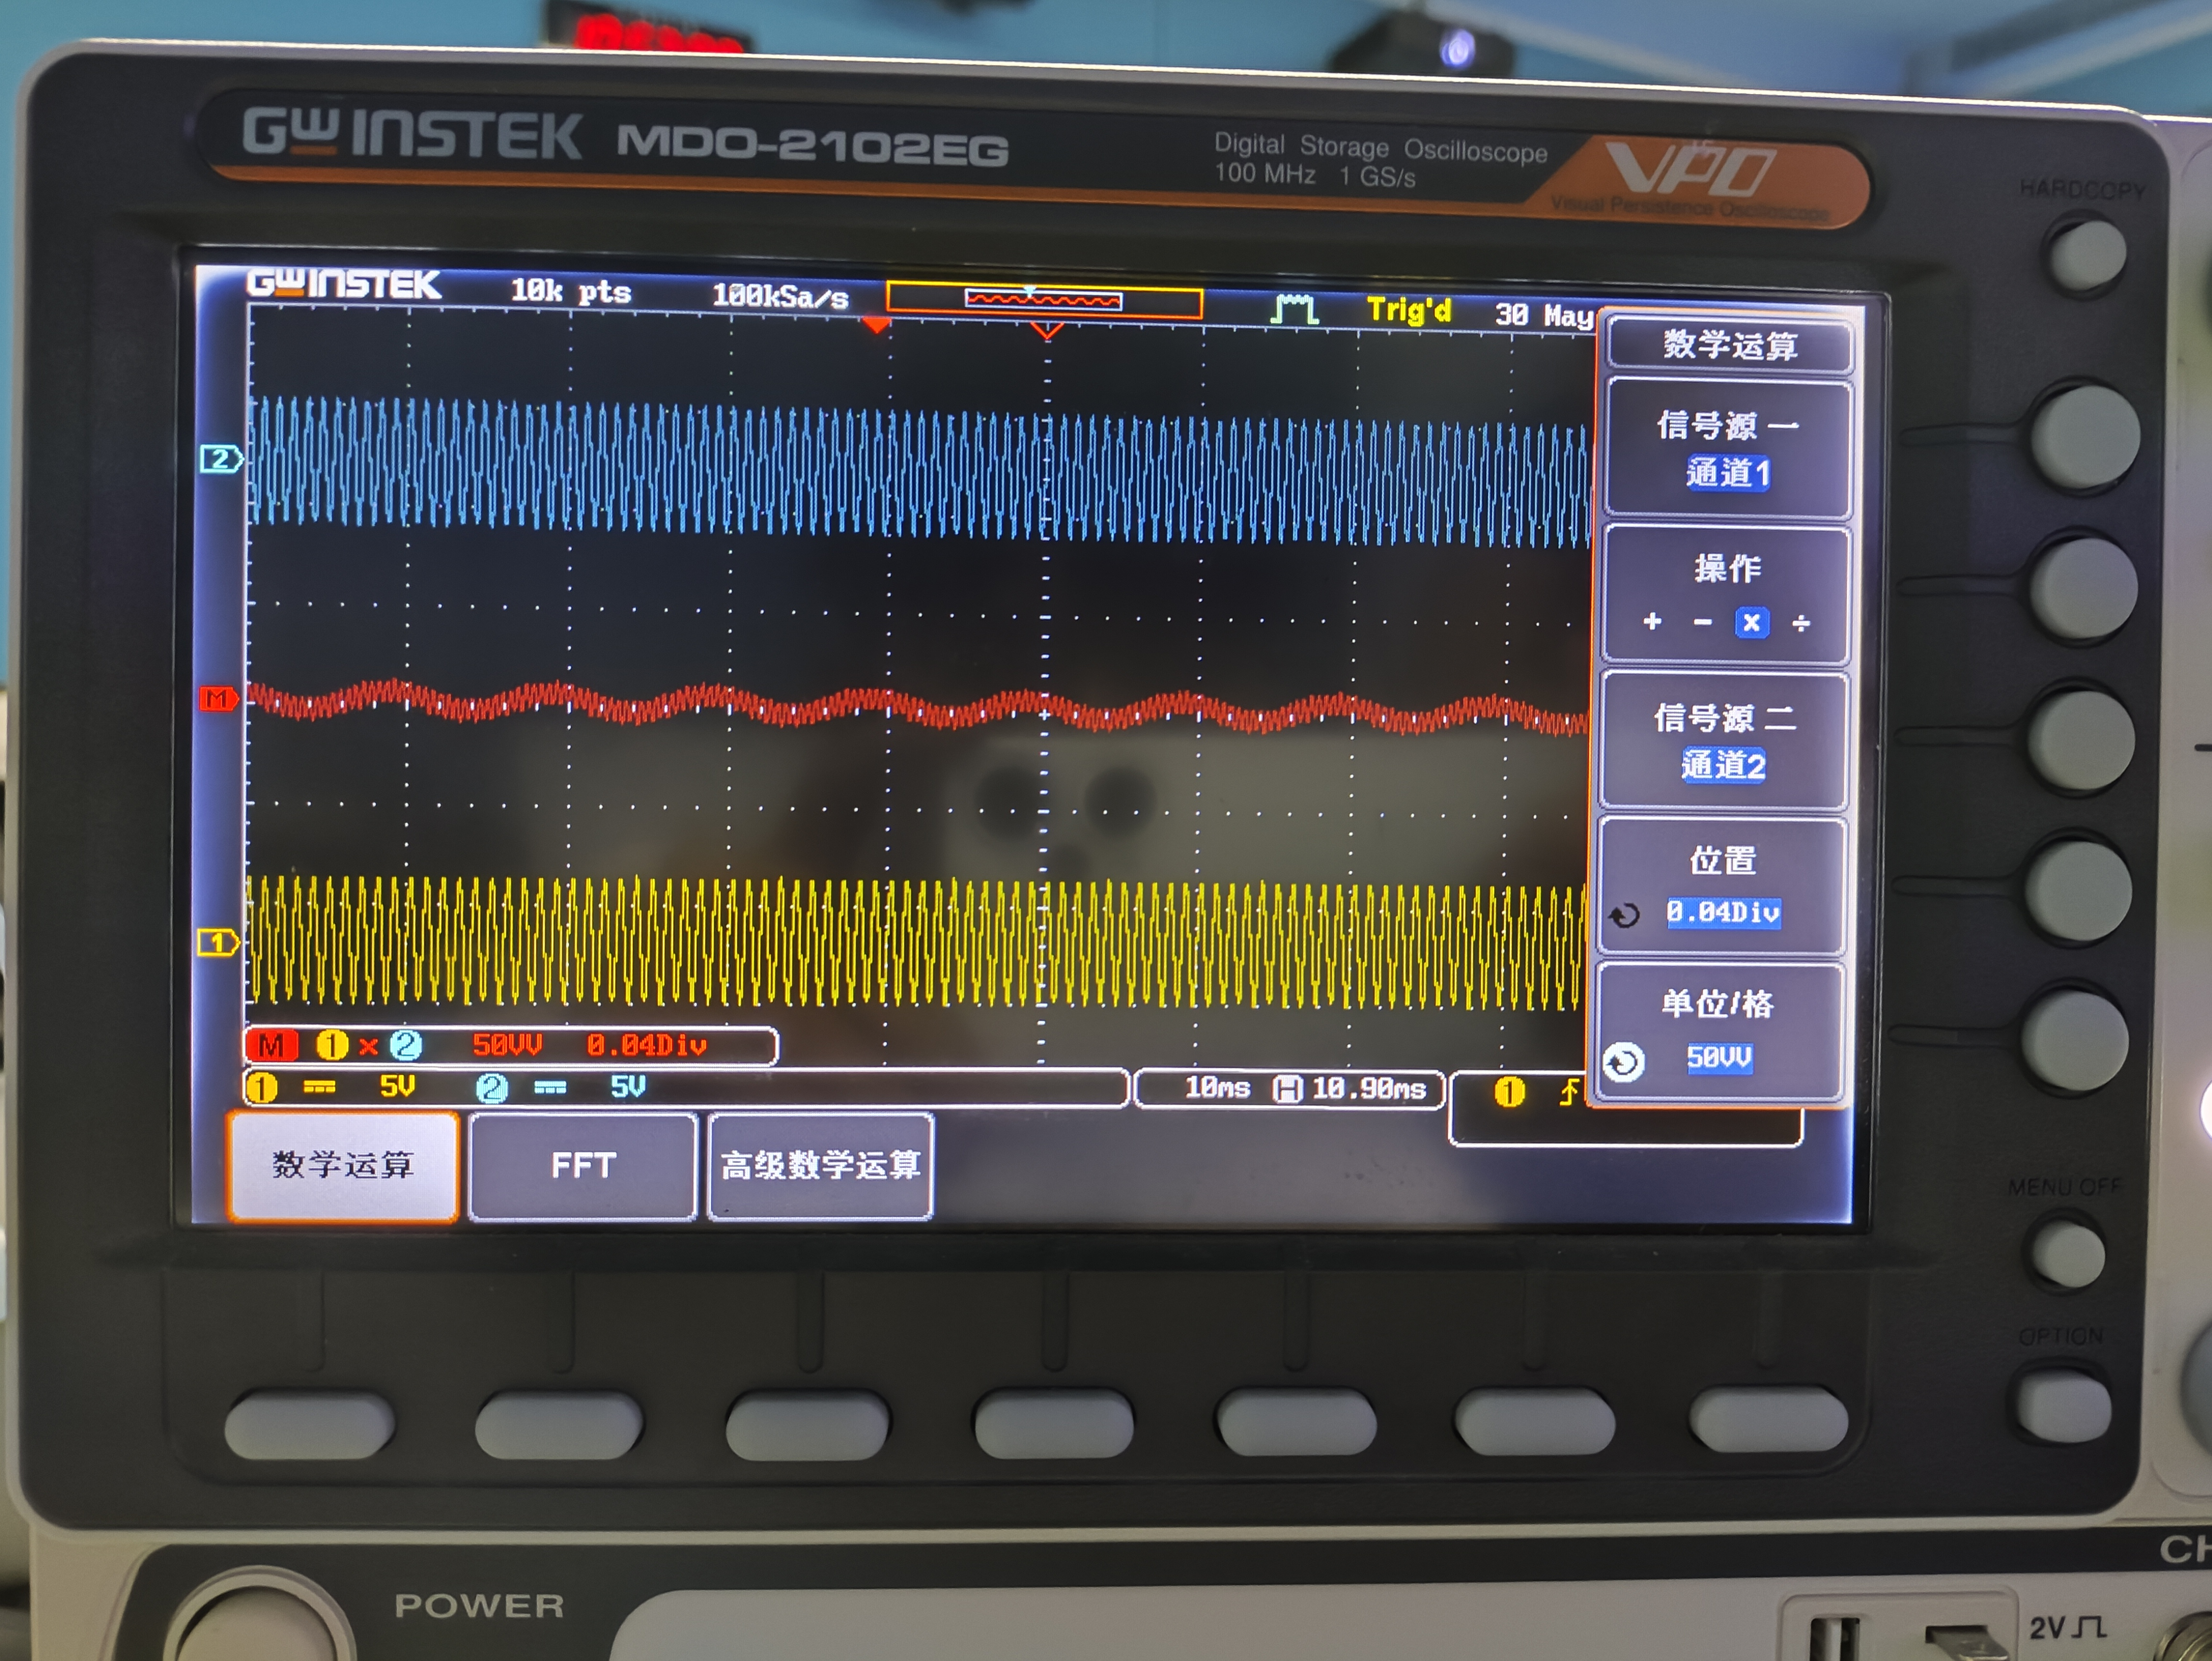
\includegraphics[width=0.7\textwidth]{assets/14.jpg}
    \caption{CH1×CH2 运算结果（CH1: 1 kHz, CH2: 1.10 kHz）}
    \label{fig:multiplication}
\end{figure}

令
\[
x_1(t)=A_1\sin(2\pi f_1 t),\quad
x_2(t)=A_2\sin(2\pi f_2 t),\quad
A_1=A_2=1.5\text{ V},\quad
f_1=1\,\text{kHz},\quad f_2=1.10\,\text{kHz}.
\]
则相乘得
\begin{align*}
x_1(t)\,x_2(t)
&=A_1A_2\,\sin(2\pi f_1 t)\,\sin(2\pi f_2 t)\\
&=\frac{A_1A_2}{2}
  \Bigl[\cos\bigl(2\pi(f_1-f_2)t\bigr)
      -\cos\bigl(2\pi(f_1+f_2)t\bigr)\Bigr]\\
&=\frac{1.5\times1.5}{2}
  \Bigl[\cos\bigl(2\pi\cdot0.10\,\mathrm{kHz}\,t\bigr)
      -\cos\bigl(2\pi\cdot2.10\,\mathrm{kHz}\,t\bigr)\Bigr]\\
&=1.125\;\bigl[\cos(2\pi\cdot100\,\mathrm{Hz}\,t)
             -\cos(2\pi\cdot2.10\,\mathrm{kHz}\,t)\bigr].
\end{align*}
因此产生了 100 Hz 的差频分量和 2.1 kHz 的和频分量，实验中主要观测到 100 Hz 差频，符合理论分析。
\vspace{0.3cm}

\textbf{六、结论和讨论}

通过本次实验，成功掌握了GDS-1102B数字示波器的基本操作方法，包括自动设置功能的使用、触发条件的调节、垂直和水平控制参数的设置等。

\vspace{0.3cm}

实验验证了数字示波器的数学运算功能，通过加法运算观察到了两个频率相近信号叠加产生的拍频现象，通过乘法运算验证了信号调制的基本原理。
\end{document}
